\documentclass[12pt]{article}
\usepackage[margin=2cm]{geometry}

% for links
\usepackage{hyperref}

% to include images
\usepackage{graphicx}

% for equation environments
\usepackage{amsmath}

% For header and footer
\usepackage{fancyhdr}
\usepackage{float} % formats figures
\pagestyle{fancy}
\fancyhf{} % clears default style
\lhead{F21BC Biologically Inspired Computation}
\lfoot{Kyle Mckay (km2008), Lina Rietuma (lr2004)}
\cfoot{\thepage}
\rfoot{HWU Person IDs: H00358352, H00361943}
\renewcommand{\headrulewidth}{0pt}

% No paragraph indentation
\setlength\parindent{0pt}
\setlength\parskip{1em}
\raggedright

\begin{document}

\title{Particle Swarm Optimisation-trained Artificial Neural Network Implementation}

\begin{center}
  \Large{Particle Swarm Optimisation-trained Artificial Neural Network Implementation}
\end{center}

\vspace{-2em}
\section{Introduction}
%\vspace{-1.5em}

The following specifies the implementation of a particle swarm
optimisation (PSO) algorithm and its subsequent use in training an
artificial neural network (ANN) to fit a binary classification dataset.
PSO hyperparameters are investigated in an effort to improve search
space exploration and thus classification performance. Finally, PSO is compared to back-propagation as an alternative approach for ANN training and solving the given classification problem.

\vspace{-1.5em}
\section{Program development rationale}
%\vspace{-1.5em}

Following on from the ANN implementation, PSO was also implemented in
Python using NumPY for efficient updates to all position and velocity
dimensional components at once.

The implementation consists of a \texttt{particle} class which houses the
particle specific instance data (position, velocity, informants and best position found) and the
methods used to perform position and velocity updates. The \texttt{swarm}
class is used to instantiate a new PSO swarm with a defined set of search space
dimensions; modify the PSO hyperparameters; and ultimately initiate a search.

For quality of life, the fitness function used by the search is a parameter
and not hard-coded into the swarm class. This means the PSO code is not coupled
to a specific search problem and is more generally usable. By default,
the sphere function is used for fitness since it works in \(n\) dimensions
and is a simple test case.

The swarm particles are initialised uniformly throughout the search space
by distributing a shared uniform vector of values and their initial velocities
are set in accordance with SPSO 2011 \cite{Clerc}. A ring topology \cite{Clerc} is used to ensure
there is an adequate level of overlapping linkage for information to propagate through
the swarm.

During the search, the "absorbing" \cite{Chu} boundary enforcement scheme is used
for simplicity. Other schemes were tried (random, reflecting) and found to have
little effect.

For use in investigation, a static \texttt{from\_list} method is added to
the \texttt{network} class that converts an appropriate length \texttt{numpy.ndarray}
into a \texttt{network} instance. In this way, a particle's current position
represents an ANN that can be used with the dataset to produce a fitness value (loss, accuracy, etc.)


\vspace{-1.5em}
\section{Methods}
%\vspace{-1.5em}

To ensure a fair comparison between back-propagation and PSO models, the same baseline architecture of 2 layers with 4 nodes each is used. To find the optimal PSO configuration the following hyper-paramters were formally investigated - swarm size, search space range, inertia weight, beta, gamma, and epsilon values. Additionally, different deltas, numbers of iterations, fitness metrics and search problems were explored in an attempt to improve PSO's performance.

Swarm sizes are tested in the range from 10 to 100 particles. The optimal swarm size is problem-dependent, heavily influenced by the dimensionality of the problem \cite{Razee}. Larger swarms are more effective at finding global minima in complex problem landscapes but come with additional computational complexity. In the older PSO implementations, \(S = 10 + 2\sqrt{D}\) is a suggested approach for determining the optimal swarm size (implies a swarm of 24 particles for the dimensionality of this problem) while newer implementations advise using 40 particles \cite{Clerc}.

Inertia weight determines the proportion of the original velocity to be retained with suggested values ranging from minimum value between 0.2 and 0.4, the maximum between 0.9 and 1.2 \cite{Razee} \cite{Gudise}, hence the decision to test values around this range.

Gudise et al (2003) suggests that an overly restricted search space (e.g. in the range -1 to 1) prevents particles from finding the global minima and finds rapid improvements in the time to convergence as the search range is increased, with optimal range (-100, 100) \cite{Gudise}. From experiments with back-propagation models, it was known that most weight values are within (-1, 1) range, therefore a search space of (-100, 100) might be an overestimate for the given problem, nonetheless guided the choice for search ranges to test.

\vspace{-1.5em}
\section{Results}
%\vspace{-1.5em}


\begin{figure}[H]
  \centering
  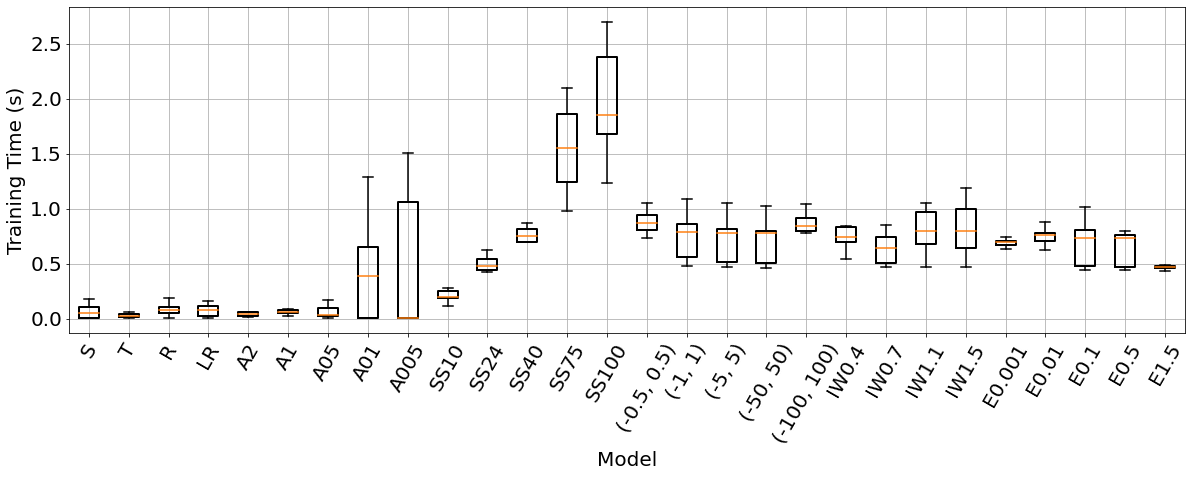
\includegraphics[width=1\textwidth]{figs/combo_ttime.png}
  \caption{
    Average training time of each model across 10 iterations.
    Modified hyperparameter abbreviation identifies each model:
    L = hidden layers, N = nodes, S|T|R|LR = activation function,
    A = learning rate for back-propagation models, SS = swarm size, () = search range, IW = inertia weight, E = epsilon for PSO models.
  }
  \label{fig:ttime}
\end{figure}

\begin{figure}[H]
  \centering
  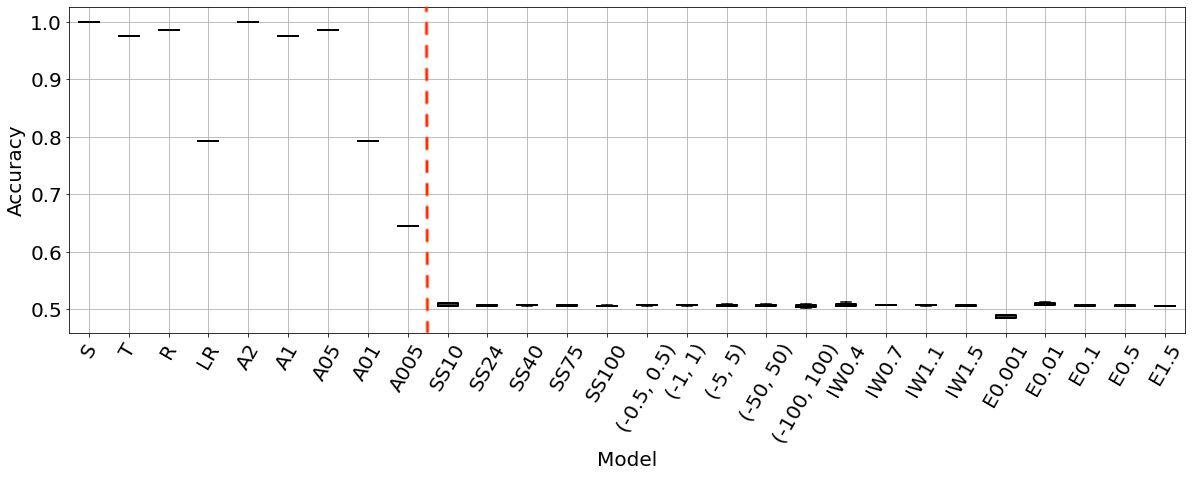
\includegraphics[width=1\textwidth]{figs/combo_acc.png}
  \caption{
    Average accuracy of each model across 10 iterations.
    Modified hyperparameter abbreviation identifies each model:
    L = hidden layers, N = nodes, S|T|R|LR = activation function,
    A = learning rate for back-propagation models, SS = swarm size, () = search range, IW = inertia weight, E = epsilon for PSO models.
  }
  \label{fig:accuracy}
\end{figure}

Expectedly, a more complex PSO implementations increases ANN's training time (Figure \ref{fig:ttime}).

PSO-trained ANNs are evidently underperforming compared to back-propagation models, with top accuracy of $\sim$51\% (Figure \ref{fig:accuracy}). Similarly low accuracies, regardless of PSO hyper-parameter combination used, suggest that PSO particles easily get stuck in a local optima.

To improve PSO's performance, alternative fitness metrics were tested. A switch from classification accuracy to cross-entropy loss value was made to capture a more detailed change in ANN's performance as the particles move through search space.  An observation that all input instances are classified as the dominant class (i.e., the class with more instances) motivated the switch to a fitness metric insensitive to class size  imbalances, i.e. Matthew's Correlation Coefficient (MCC). Using MCC prevents classifying all inputs as a single class, however the overall accuracy decreased.


A relatively large Beta with respect to Gamma can result in excessive wandering within the problem space while the reverse  can lead to the swarm prematurely settling on a local minimum. Approximately equal values of Beta and Delta yield the most effective search of the problem space \cite{Kennedy}.

Particles' step size is most commonly set to 1 \cite{Luke}.


PSO's seeming lack of responsiveness to any hyper-parameter changes, prevents from making any meaningful conclusions about the importance of optimal hyper-paramter combinations in the algorithm's performance - any effects are cancelled out by the swarm getting bound to a local optima. Despite research evidence of PSOs being as efficient if not better at finding optimum weights than backpropagation and PSO trained ANNs generalising better to unseen data \cite{Kennedy}, our results do not support the same conclusion. Based on the classification accuracy and the increased training time, back-propagation is by far a better approach for ANN training for the given classification problem.

In retrospect, enforcing boundaries for velocity values ..

\vspace{-1.5em}
\begin{thebibliography}{10}

\bibitem{Chu} W. Chu, X. Gao, S. Sorooshian, 2011, ``Handling boundary constraints for particle swarm optimization in high-dimensional search space'', doi: 10.1016/j.ins.2010.11.030
\bibitem{Luke} Sean Luke, 2013, ``Essentials of Metaheuristics", Lulu, second edition, available at http://cs.gmu.edu/∼sean/book/metaheuristics/
\bibitem{Kennedy} J. Kennedy, R. Eberhart, 1995, ``Particle swarm optimization," Proceedings of ICNN'95 - International Conference on Neural Networks,  pp. 1942-1948 vol.4, doi: 10.1109/ICNN.1995.488968.
\bibitem{Razee} A. Rezaee Jordehi, J. Jasni, 2013, ``Parameter selection in particle swarm optimisation: a survey, Journal of Experimental \& Theoretical Artificial Intelligence", 25:4, 527-542, DOI: 10.1080/0952813X.2013.782348
\bibitem{Clerc} Maurice Clerc, 2012, ``Standard Particle Swarm Optimisation", hal-00764996
\bibitem{Gudise}  V. G. Gudise, G. K. Venayagamoorthy, 2003, ``Comparison of particle swarm optimization and backpropagation as training algorithms for neural networks," Proceedings of the 2003 IEEE Swarm Intelligence Symposium. SIS'03 (Cat. No.03EX706), pp. 110-117, doi: 10.1109/SIS.2003.1202255.


\end{thebibliography}

\end{document}
